%\section{Introduction}
\label{remy:intro}

Is it possible for a computer to ``discover'' the right rules for
congestion control in heterogeneous and dynamic networks? Should
computers, rather than humans, be tasked with developing congestion
control methods?  And just how well can we make computers perform this
task?

We investigated these questions and found that computers can design
schemes that in some cases surpass the best human-designed methods to
date, when supplied with the appropriate criteria by which to
judge a congestion-control algorithm. We attempt to probe the limits
of these machine-generated protocols, and discuss how this style of
transport-layer protocol design can give more freedom to network
architects and link-layer designers.

\begin{figure}
\vspace{\baselineskip}
\begin{centering}
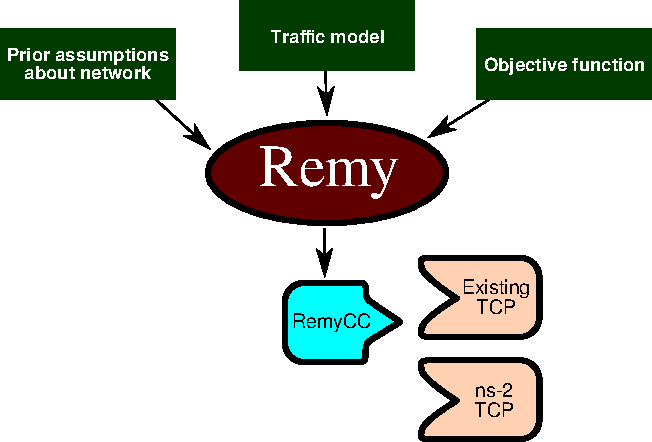
\includegraphics[width=0.75 \columnwidth]{remy.pdf}
\caption{Remy designs congestion-control schemes automatically to
  achieve desired outcomes. The algorithms it produces may replace
the congestion-control module of a TCP implementation, and fit into
a network library or kernel module that implements congestion
control (DCCP, SCTP, the congestion manager, application-layer
transmission control libraries, ns-2 modules, etc.).}

\end{centering}

\end{figure}

Congestion control, a fundamental problem in multi-user computer
networks, addresses the question: when should an endpoint transmit
each packet of data? An ideal scheme would transmit a packet whenever
capacity to carry the packet was available, but because there are many
concurrent senders and the network experiences variable delays, this
question isn't an easy one to answer. On the Internet, the past thirty
years have seen a number of innovative and influential answers to this
question, with solutions embedded at the endpoints (mainly in TCP)
aided occasionally by queue management and scheduling algorithms in
bottleneck routers that provide signals to the endpoints.

This area has continued to draw research and engineering effort
because new link technologies and subnetworks have proliferated and
evolved. For example, the past few years have seen an increase in
wireless networks with variable bottleneck rates; datacenter networks
with high rates, short delays, and correlations in offered load; paths
with excessive buffering (now called ``bufferbloat''); cellular
wireless networks with highly variable, self-inflicted packet delays;
links with non-congestive stochastic loss; and networks with large
bandwidth-delay products. In these conditions, the classical
congestion-control methods embedded in TCP can perform poorly, as many
papers have shown (\S\ref{remy:related}).

%Although the control methods in TCP have evolved over the past several
%years (indeed, there is no longer just one TCP scheme in practice),
%they are generally rooted in an implicit assumption that the Internet
%exhibits the same behaviors that it did in the 1980s. Classical TCP
%uses only three congestion signals: packet losses (assumed to be
%caused by buffer losses), the smoothed round-trip time (RTT), and the
%delay jitter (assumed to be a lightly-tailed
%distribution)~\cite{Jacobson88}. Newer phenomena, such as stochastic
%packet loss or heavy-tailed jitter, are not easily accounted for.

Without the ability to adapt its congestion-control algorithms to new
scenarios, TCP's inflexibility constrains architectural evolution, as
we noted in an earlier position paper~\cite{hotnets2011}. Subnetworks
and link layers are typically evaluated based on how well TCP performs
over them.  This scorecard can lead to perverse behavior, because
TCP's network model is limited. For example, because TCP assumes that
packet losses are due to congestion and reduces its transmission rate
in response, some subnetwork designers have worked hard to hide
losses. This often simply adds intolerably long packet delays. One may
argue that such designs are misguided, but the difficulties presented
by ``too-reliable'' link layers have been a perennial challenge for 25
years~\cite{Clark88} and show no signs of abating. With the rise of
widespread cellular connectivity, these behaviors are increasingly
common and deeply embedded in deployed infrastructure.

The designers of a new subnetwork may well ask what they should do to
make TCP perform well. This question is surprisingly hard to answer,
because the so-called teleology of TCP is unknown: exactly what
objective does TCP congestion control optimize? TCP's dynamic
behavior, when competing flows enter and leave the network, remains
challenging to explain~\cite{slowcc}.  In practice, the need to ``make
TCP perform well'' is given as a number of loose guidelines, such as
IETF RFC 3819~\cite{rfc3819}, which contains dozens of pages of
qualitative best current practice. The challenging and subtle nature
of this area means that the potential of new subnetworks and network
architectures is often not realized.

\subsection*{Design overview}

How should we design network protocols that free subnetworks and links
to evolve freely, ensuring that the endpoints will adapt properly
\emph{no matter what} the lower layers do?  We believe that the best
way to approach this question is to take the design of specific
algorithmic mechanisms out of the hands of human designers (no matter
how sophisticated!), and make the end-to-end algorithm be a function
of the desired overall behavior.

%These actions should not
%depend on explicit signals about unusual network behaviors, e.g., if a
%new network were to reorder packets because of multi-path routing,
%endpoints should not have to be notified.

We start by explicitly stating an {\em objective} for congestion
control; for example, given an unknown number of users, we may
optimize some function of the per-user throughput and packet delay, or
a summary statistic such as average flow completion time. Then,
instead of writing down rules by hand for the endpoints to follow, we
start from the desired objective and work backwards in three steps:

%\item We specify a utility function that quantifies the
%  benefit to each user of the network. As in other work, this is
%  generally a concave function of average throughput, so that a fair
%  allocation is preferred. We then subtract a concave function of the
%  user's average delay, to penalize induced latency.

%We have developed an alternate approach for end-to-end resource
%management and transmission control. 

\begin{enumerate}

\item First, model the protocol's prior assumptions about the network;
  i.e., the ``design range'' of operation. This model
  may be different, and have different amounts of uncertainty, for a
  protocol that will be used exclusively within a data center,
  compared with one intended to be used over a wireless link or one
  for the broader Internet. A typical model specifies upper and lower
  limits on the bottleneck link speeds, non-queueing delays, queue
  sizes, and degrees of multiplexing.
%The model represents the
%  designer's prior knowledge about the networks that the protocol will
%  encounter.

\item Second, define a traffic model for the offered load given to
  endpoints. This may characterize typical Web traffic, video
  conferencing, batch processing, or some mixture of these. It may
  be synthetic or based on empirical measurements.

\item Third, use the modeled network scenarios and traffic to design a
  congestion-control algorithm that can later be executed on endpoints.

\end{enumerate}

We have developed an optimization tool called Remy that takes these
models as input, and designs a congestion-control algorithm that tries
to maximize the total expected value of the objective function, measured over the set of
network and traffic models. The resulting pre-calculated, optimized
algorithm is then run on actual endpoints; no further learning happens
after the offline optimization. The optimized algorithm is run as part
of an existing TCP sender implementation, or within any
congestion-control module. No receiver changes are necessary (as of
now).

\subsection*{Summary of results}

We have implemented Remy. Running on a 48-core server at MIT, Remy
generally takes a few hours of wall-clock time (one or two CPU-weeks)
to generate congestion-control algorithms offline that work on a wide
range of network conditions.

Our main results from several simulation experiments
with Remy are as follows:

\begin{enumerate}

\item For networks broadly consistent with the assumptions provided to
  Remy at design time, the machine-generated algorithms dramatically
  outperform existing methods, including TCP Cubic, Compound TCP, and
  TCP Vegas.

\item Comparing Remy's algorithms with schemes that require
  modifications to network gateways, including Cubic-over-sfqCoDel and
  XCP, Remy generally matched or surpassed these schemes, despite
  being entirely end-to-end.

\item We measured the tradeoffs that come from specificity in the
  assumptions supplied to Remy at design time. As expected,
  more-specific prior information turned out to be helpful when it was
  correct, but harmful when wrong. We found that RemyCC schemes
  performed well even when designed for an order-of-magnitude
  variation in the values of the underlying network parameters.
\end{enumerate}

%\subsection*{Outline}

% We describe our model of the problem in \S~\ref{model}, and the design
% of Remy's optimizer in \S~\ref{design}. In \S~\ref{eval}, we describe
% the results of a series of ns-2 simulations that compared Remy's
% algorithms to the best human-designed congestion-control
% algorithms. We found that, for networks whose parameters fall within
% the range of those provided to Remy at optimization time, the
% resulting computer-generated algorithm conclusively outforms existing
% methods, including TCP Cubic and Vegas.

% We also compared Remy's algorithms with more intrusive schemes that
% require modifications to network gateways, including
% Cubic-over-sfqCoDel and XCP. Remy also outperformed or matched these
% schemes, despite being entirely end-to-end.

% A significant concern with any machine-learned method is its
% generalizability to situations not seen during training.\footnote{The
%   same risk of overfitting may arguably apply to human-designed
%   algorithms. For example, traditional congestion control was built on
%   the assumption that even when a gateway buffer is full enough that
%   it is dropping packets, the induced queueing delay is still
%   acceptable to other users. On contemporary network paths that do not
%   meet this constraint, including wireless links and ``bufferbloated''
%   home connections, TCP performs poorly. However, the problem of
%   overfitting is generally thought to be more acute with computer-designed
%   methods.} We attempt to characterize this phenomenon as it
% applies to Remy by measuring its performance as we vary network
% parameters to fall further and further outside the range seen during
% training.

On a simulated 15~Mbps fixed-rate link with eight senders contending and
an RTT of 150~ms, a computer-generated congestion-control algorithm
achieved the following improvements in median throughput and
reductions in median queueing delay over these existing protocols:

{\footnotesize
\begin{tabular}{|l|c|c|}
\hline
Protocol & Median speedup & Median delay reduction \\
\hline
\hline
Compound & $2.1\times$ & $2.7\times$ \\
NewReno & $2.6\times$ & $2.2\times$ \\
Cubic & $1.7\times$ & $3.4\times$ \\
Vegas & $3.1\times$ & $1.2\times$ \\
\hline
Cubic/sfqCoDel & $1.4\times$ & $7.8\times$ \\
XCP & $1.4\times$ & $4.3\times$ \\
\hline
\end{tabular}
}

In a trace-driven simulation of the Verizon LTE downlink with four
senders contending, the \emph{same} computer-generated protocol achieved these
speedups and reductions in median queueing delay:

{\footnotesize
\begin{tabular}{|l|c|c|}
\hline
Protocol & Median speedup & Median delay reduction \\
\hline
\hline
Compound & $1.3\times$ & $1.3\times$ \\
NewReno & $1.5\times$ & $1.2\times$ \\
Cubic & $1.2\times$ & $1.7\times$ \\
Vegas & $2.2\times$ & $0.44\times \downarrow$ \\
\hline
Cubic/sfqCoDel & $1.3\times$ & $1.3\times$ \\
XCP & $1.7\times$ & $0.78\times \downarrow$ \\
\hline
\end{tabular}
}

The source code for Remy, our ns-2 models, and the algorithms that Remy
designed are available from \mbox{\url{http://web.mit.edu/remy}}.
